\documentclass[10pt,conference]{IEEEtran}

\usepackage{amsmath,amssymb,amsfonts}
\usepackage{graphicx}
\usepackage{textcomp}
\usepackage{xcolor}
\usepackage{cite}
\usepackage{booktabs}
\usepackage{array}
\usepackage{url}
\usepackage{tikz}
\usetikzlibrary{shapes.geometric,arrows.meta,positioning}

\def\BibTeX{{\rm B\kern-.05em{\sc i\kern-.025em b}\kern-.08em
    T\kern-.1667em\lower.7ex\hbox{E}\kern-.125emX}}

\begin{document}

\title{Pool Size, Not Fusion Rule: A Corrected Evaluation of Rank Fusion versus Linear Fusion for Knowledge-Graph-Reranked Medical Retrieval}

\author{
\IEEEauthorblockN{Dhairya Panwar}
\IEEEauthorblockA{Department of Computer Science \\
\textit{Sharda University} \\
Email: 2023243674.dhairya@ug.sharda.ac.in}
\and
\IEEEauthorblockN{Aryan Raosaheb Doule}
\IEEEauthorblockA{Department of Computer Science \\
\textit{Sharda University} \\
Email: 2023215705.aryan@ug.sharda.ac.in}
}

\maketitle

\begin{abstract}
Retrieval-augmented medical question-answering systems that combine lexical, dense, and knowledge-graph evidence typically fuse these signals either through a linear weighted sum or through a rank-based fusion rule followed by structured reranking. In an earlier phase of this project, evaluated under a protocol later found to share 58 of 82 confirmatory test rows with the pool used to build the retrieval index, we reported that a grid-searched linear-fusion baseline (CRFS) degenerates to zero weight on both dense retrieval and source recency, and that a proposed reciprocal-rank-fusion (RRF) pipeline that structurally protects each signal's role corrects this failure and improves accuracy. Under a corrected, leak-free protocol, with a frozen test set (n=123: 41 canonical and 82 lay-paraphrased queries across 41 conditions) constructed as the exact row-level complement of the tuning pool, this finding does not replicate. The re-tuned CRFS weights, $(w_{\text{BM25}}, w_{\text{dense}}, w_{\text{KG}}, w_{\text{rec}}) = (0.205, 0.314, 0.378, 0.103)$, assign meaningful weight to every signal, and CRFS (87.80\% accuracy) now outperforms the proposed pipeline (80.49\%), a gap that is nominally significant under an uncorrected pairwise test (McNemar exact $p=0.0225$) but does not survive Bonferroni correction across our four pre-registered comparisons ($\alpha=0.0125$). A dedicated attribution ablation isolates the cause: restricting CRFS to the same top-3 candidate shortlist the proposed pipeline uses reproduces the proposed pipeline's exact accuracy, with the two configurations disagreeing on only 2 of 123 queries in opposite directions ($p=1.0$), while restricting only the candidate pool with fusion rule held fixed costs 6.5 accuracy points and is itself significant ($p=0.0215$). The gap between the two architectures is therefore attributable to candidate-pool size, not to reciprocal rank fusion outperforming linear fusion; at matched pool size the two fusion rules are statistically indistinguishable. The proposed pipeline remains substantially cheaper (21.25~ms vs.\ 72.66~ms mean latency, a 3.4$\times$ reduction), because it scores knowledge-graph relevance and recency over a 3-document shortlist rather than the full 104-passage corpus: a genuine accuracy-latency trade-off, rather than the elimination of wasted computation on a zero-weight term, as we had previously and incorrectly concluded. We report this non-replication, the corrected results, and the attribution analysis that explains it, transparently.
\end{abstract}

\begin{IEEEkeywords}
information retrieval, reciprocal rank fusion, knowledge graphs, dense retrieval, medical question answering, retrieval-augmented generation, replication
\end{IEEEkeywords}

\section{Introduction}

Health information systems that answer symptom-related questions face a narrower and more consequential version of a familiar information retrieval problem: the system must rank relevant evidence highly from a small, carefully sourced corpus, where an incorrect top result carries real cost. Large language models alone are a poor fit here, since an unconstrained generative model has no mechanism to distinguish a well-supported clinical statement from a fluent but unverified one. Retrieval-augmented generation addresses this by grounding responses in retrieved text, and recent medical chatbot systems have converged on hybrid retrieval, combining lexical matching, dense semantic search, and structured knowledge such as symptom-disease graphs, to make that grounding reliable \cite{lachenmayer2026,shin2025,nikam2024}.

This paper is a corrected report on a specific design question within that hybrid-retrieval space: whether combining these signals through a linear weighted sum or a rank-based fusion rule with structured reranking is the more reliable architecture. An earlier phase of this project answered that question by observing that a grid-searched linear-fusion baseline, CRFS, converged during tuning to zero weight on both dense retrieval and source recency, and concluded that linear fusion has a structural tendency to discard useful signals under a saturating validation search. A subsequent audit found that the frozen test set used to report that result shared 58 of its 82 rows with the pool used to build the retrieval index and knowledge graph, leakage severe enough that we no longer consider any result under that protocol reliable, including the weight-collapse finding itself.

This paper reports what we found after repairing that protocol. The weight collapse does not reproduce, the accuracy ordering between the two architectures reverses, and the true source of the remaining performance gap is not the one we originally proposed. Our contributions:

\begin{enumerate}
\item We disclose the train/test leakage in our original protocol and its repair: a frozen test set as the exact complement of the tuning pool.
\item We show the CRFS weight search no longer collapses once this leak is removed: all four signals receive meaningful, nonzero weight, contradicting our original report.
\item CRFS now outperforms the proposed RRF pipeline (87.80\% vs.\ 80.49\%), reversing our original ordering, though the gap does not survive correction for multiple comparisons.
\item A dedicated ablation isolates the cause as candidate-pool size, not fusion-rule choice: at matched pool size, linear and reciprocal rank fusion are statistically indistinguishable.
\item The proposed pipeline's latency advantage persists and is legitimate, a consequence of reranking fewer candidates, not wasted zero-weight computation as we originally reported.
\item We present the resulting accuracy-latency trade-off honestly, and report the non-replication as a primary result rather than an incidental caveat.
\end{enumerate}

\section{Related Work}

Retrieval-augmented generation anchors a language model's output in retrieved evidence rather than parametric memory, and is the standard mitigation for hallucination in medical question answering \cite{lewis2020rag}. Early medical RAG systems paired parameter-efficient fine-tuning with retrieval to reduce confidently incorrect answers on constrained hardware \cite{bora2024}, and domain-specialized systems show grounding in a curated, disease-specific corpus outperforms general-purpose retrieval even with the same underlying model \cite{shin2025}. Flat, similarity-only retrieval cannot distinguish an authoritative, recent guideline from an outdated reference; hierarchical, evidence-prioritized reranking has been proposed as a correction \cite{lachenmayer2026}. Our reranking follows this reasoning but reranks by structured symptom-disease relevance rather than guideline hierarchy.

Knowledge graphs have been used to constrain generative medical systems to relationships actually present in a curated ontology, preventing invented symptom-disease associations \cite{nikam2024}. We adopt the same guardrail principle but apply it as a reranking signal over a recalled shortlist rather than a standalone scoring source. Safety-oriented evaluation frameworks for medical dialogue systems argue accuracy alone understates risk and that explicit, multi-dimensional evaluation is necessary for trust \cite{putra2025}; our use of paired significance testing, bootstrap confidence intervals \cite{efron1993bootstrap}, and Wilson intervals follows the same spirit. Offline, edge-deployable medical assistants show low-latency inference is achievable without cloud dependency \cite{ruhland2026}, motivating our decision to report latency as a primary result.

At the retrieval-mechanics level, our architecture builds on three established techniques. BM25 remains a strong, well-understood lexical baseline \cite{robertson2009bm25}. Dense retrieval with transformer bi-encoders captures semantic similarity lexical matching misses \cite{karpukhin2020dpr}, and biomedical dense encoders trained on PubMed search-relevance signal substantially outperform general-purpose sentence encoders on medical retrieval \cite{jin2023medcpt}, which is why we use such an encoder rather than a general-domain one \cite{devlin2019bert,reimers2019sbert}. Reciprocal rank fusion combines ranked lists from heterogeneous retrievers without requiring comparable raw score scales, and outperforms both individual rankers and more elaborate learned combination methods in general-purpose retrieval \cite{cormack2009rrf}. To our knowledge it has not previously been evaluated for its sensitivity to candidate-pool size relative to a linear-fusion baseline in medical retrieval-fusion, which is the comparison this paper reports.

\section{System Architecture}
\label{sec:architecture}

The system retrieves supporting evidence from a corpus of short clinical guideline excerpts and returns the disease whose evidence best matches a free-text symptom description. Two architectures are compared throughout this paper: a linear score-fusion baseline (Section~\ref{ssec:crfs}), which represents the design we started with, and the proposed rank-fusion-then-rerank pipeline (Section~\ref{ssec:proposed}), which we set out to replace it with. Two additional configurations, described in Section~\ref{ssec:attribution}, isolate which architectural choice is responsible for the gap between them.

\subsection{Linear Fusion Baseline (CRFS)}
\label{ssec:crfs}

The baseline computes four per-document scores, min-max normalized BM25 score, min-max normalized dense cosine similarity, a knowledge-graph relevance score, and a recency score from the guideline's source date, and combines them as
\begin{equation}
\text{CRFS}(d) = w_1 s_{\text{BM25}}(d) + w_2 s_{\text{dense}}(d) + w_3 s_{\text{KG}}(d) + w_4 s_{\text{rec}}(d),
\label{eq:crfs}
\end{equation}
with weights selected by grid search on a held-out validation split, constrained to a 4-simplex ($\sum_i w_i = 1$, $w_i \geq 0$). The knowledge-graph relevance score is computed independently of the preliminary lexical or dense prediction: it extracts symptom mentions from the query, compares them against each candidate disease's known symptom set in a graph built from disease-symptom co-occurrence, and weights each shared symptom by an inverse-document-frequency-style specificity term so rare, more diagnostic symptoms count more than common ones. This scoring mechanism is identical between the two architectures; what changes is how the resulting signal, and how many candidate documents, participate in the final ranking.

\subsection{Proposed Architecture (RRF + KG + Recency)}
\label{ssec:proposed}

\begin{figure}[t]
\centering
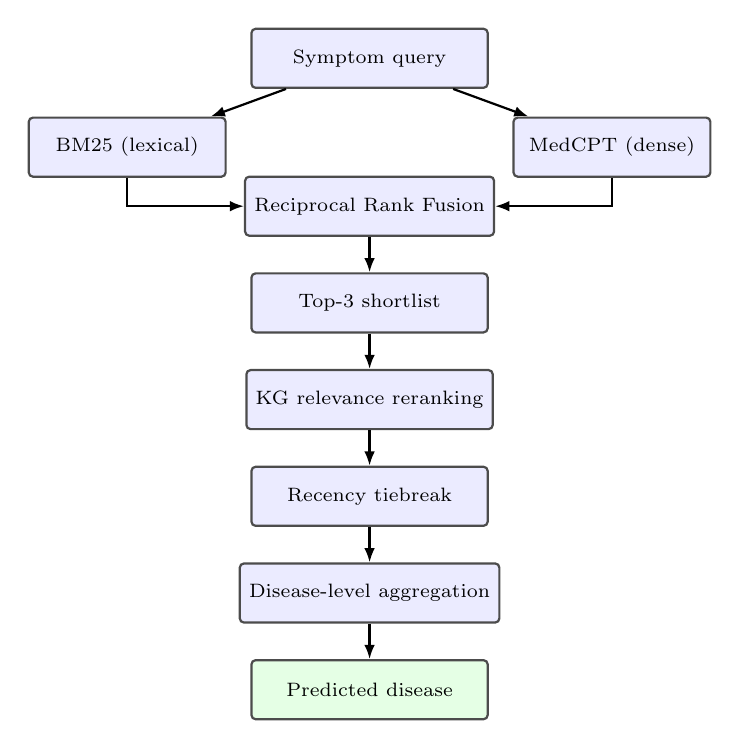
\begin{tikzpicture}[
  node distance=0.35cm and 0.3cm,
  box/.style={rectangle, rounded corners=1.5pt, draw=black!70, thick, fill=blue!8,
              minimum width=3.0cm, minimum height=0.75cm, align=center, font=\scriptsize},
  small/.style={box, minimum width=2.5cm},
  arrow/.style={-{Latex[length=1.8mm]}, thick}
]
\node[box] (query) {Symptom query};
\node[small, below left=of query] (bm25) {BM25 (lexical)};
\node[small, below right=of query] (dense) {MedCPT (dense)};
\node[box, below=1.1cm of query] (rrf) {Reciprocal Rank Fusion};
\node[box, below=0.45cm of rrf] (short) {Top-3 shortlist};
\node[box, below=0.45cm of short] (kg) {KG relevance reranking};
\node[box, below=0.45cm of kg] (rec) {Recency tiebreak};
\node[box, below=0.45cm of rec] (agg) {Disease-level aggregation};
\node[box, below=0.45cm of agg, fill=green!10] (pred) {Predicted disease};

\draw[arrow] (query) -- (bm25);
\draw[arrow] (query) -- (dense);
\draw[arrow] (bm25) |- (rrf);
\draw[arrow] (dense) |- (rrf);
\draw[arrow] (rrf) -- (short);
\draw[arrow] (short) -- (kg);
\draw[arrow] (kg) -- (rec);
\draw[arrow] (rec) -- (agg);
\draw[arrow] (agg) -- (pred);
\end{tikzpicture}
\caption{Proposed retrieval pipeline. Dense retrieval contributes to which documents are recalled into the shortlist (Reciprocal Rank Fusion), a stage that is separate from the reranking weight the knowledge graph receives.}
\label{fig:architecture}
\end{figure}

The proposed pipeline, shown in Fig.~\ref{fig:architecture}, separates recall from ranking rather than combining both into one weighted sum. BM25 and dense retrieval scores are first converted to ranks and combined by reciprocal rank fusion,
\begin{equation}
\text{RRF}(d) = \frac{1}{k + r_{\text{BM25}}(d)} + \frac{1}{k + r_{\text{dense}}(d)},
\label{eq:rrf}
\end{equation}
with $k=60$, the constant reported as broadly effective without per-task tuning in the original formulation \cite{cormack2009rrf}; we use this default rather than searching it. The top documents by RRF score form a shortlist; its size is the only hyperparameter selected by search in the proposed architecture, using the same protocol as the baseline (Section~\ref{ssec:tuning}). Within the shortlist, documents are reranked primarily by knowledge-graph relevance; residual ties are broken first by RRF score and then by source recency, so a more recently reviewed guideline is preferred only when two candidates are otherwise equally well supported. Because dense retrieval participates in recall through ranks rather than a scalar coefficient, a validation search over shortlist size cannot assign it zero effective contribution the way a weight search can zero out a term in Eq.~\eqref{eq:crfs}. This is a structural property of the architecture; Section~\ref{sec:results} reports whether it corresponds to a comparable empirical difference.

Both architectures conclude with the same disease-level aggregation: within the top 20 ranked documents, each candidate disease accumulates a rank-discounted sum of the scores of its supporting documents, and the highest-accumulating disease is returned as the prediction.

\subsection{Attribution Ablations (N1, N2)}
\label{ssec:attribution}

The proposed pipeline and the linear baseline differ along three axes at once: candidate-pool size, fusion rule, and whether recency acts as an additive term or a tiebreaker. Two configurations, introduced during the repair in Section~\ref{sec:dataset}, hold two axes fixed so the third can be isolated. \textbf{N1} restricts the linear baseline (Section~\ref{ssec:crfs}) to the proposed pipeline's top-3 shortlist, holding fusion rule (linear) fixed while pool size changes from the full corpus to top-3. \textbf{N2} is the proposed pipeline (Section~\ref{ssec:proposed}) with the recency tiebreak removed, holding fusion rule (RRF) and pool size (top-3) fixed. Neither was part of our original report; both test competing explanations for the CRFS-vs-proposed gap.

Retrieval is one component of a larger preliminary-guidance assistant that also includes a triage-urgency classifier and a symptom-elicitation dialogue policy, evaluated separately and outside the scope of this paper's frozen evaluation; we report only the retrieval component here, since it carries this paper's central architectural claim.

\section{Dataset and Evaluation Protocol}
\label{sec:dataset}

\subsection{Corpus and Query Construction}

Symptom-disease associations were sourced from a public dataset of 4{,}920 labeled records, which reduced to 304 unique symptom-disease rows across 41 conditions after removing exact duplicates. A guideline corpus of 104 short evidence passages was constructed from publicly available medical reference pages (MedlinePlus and CDC), covering all 41 conditions; source review dates were recovered for 73 of 104 passages (70.2\%), and the remainder are treated as undated rather than assigned a fabricated date.

Evaluation queries are short free-text symptom statements. To test whether dense retrieval's contribution is visible once it can no longer be silently removed by a weight search, we pre-specified a lay-language paraphrase dictionary (clinical-to-colloquial symptom mappings, e.g.\ ``breathlessness'' $\rightarrow$ ``can't catch my breath'') and applied it to a majority of the confirmatory test queries; this dictionary was itself audited and corrected once during the repair described below, prior to the confirmatory run reported in Section~\ref{sec:results}.

\subsection{Frozen Train/Validation/Test Protocol}
\label{ssec:protocol}

The confirmatory test set reported here (v3) consists of 123 queries, one canonical and two paraphrased per condition across all 41 conditions (41 canonical, 82 paraphrased), drawn with a fixed seed (157) as the exact row-level complement of a 181-row development pool: every row not assigned to development is assigned to test, and no row is assigned to both. This is a deliberate change from the protocol used to produce our originally reported results (v2), under which the test set (82 queries, drawn independently of the development pool's own construction) was later found, on audit, to share 58 of its 82 rows with the development pool. Because both the retrieval index and the knowledge graph are built from disease-level aggregates over the development pool, this overlap meant most confirmatory test queries corresponded to diseases whose aggregated profiles were built partly from the same rows being used to test them. We do not consider any v2 result, including the weight-collapse finding that motivated this project's original design, reliable evidence under that protocol.

Under the corrected v3 protocol, the test set and development pool are disjoint by construction. Eight conditions with insufficient rows for a meaningful validation split (AIDS, Acne, Allergy, Fungal infection, Gastroenteritis, Heart attack, Paralysis (brain hemorrhage), Urinary tract infection) were excluded specifically from the development-validation portion used to score tuning candidates; this is disclosed here rather than hidden, and does not affect the confirmatory test set, which retains all 41 conditions.

\subsection{Hyperparameter Tuning}
\label{ssec:tuning}

Hyperparameters were selected using the 181-row development pool, split internally into a tuning-train portion (used to build the retrieval index, dense embeddings, and knowledge graph) and a tuning-validation portion (used only to score candidate configurations). The CRFS weight grid search, constrained to the 4-simplex, converged to $(w_{\text{BM25}}, w_{\text{dense}}, w_{\text{KG}}, w_{\text{rec}}) = (0.205, 0.314, 0.378, 0.103)$: every signal receives meaningful, nonzero weight. This is the central departure from our originally reported result. Under the leaky v2 protocol, the identical search converged to $(0.4, 0.0, 0.6, 0.0)$, zero weight on both dense retrieval and recency, which became the basis for this project's original thesis. That configuration does not reproduce under the corrected protocol, and we no longer treat it as evidence that linear fusion has an intrinsic tendency to discard useful signals; the effect was specific to the leaky validation setup rather than a general property of the fusion rule. We lack a controlled experiment isolating exactly which mechanism connected the leakage to that degenerate solution, and flag any explanation of that mechanism as a plausible hypothesis rather than an established finding.

The RRF shortlist size, the only hyperparameter selected by search in the proposed architecture, was re-tuned over an extended grid (3, 5, 8, 10, 15, 20, 30, 50 documents) after an audit found the original grid (10, 15, 20, 30, 50) omitted values small enough to reach the true optimum. The corrected search converges to a shortlist of 3 documents, substantially smaller than the value of 15 used in our original report. We use $k=60$ throughout and do not search over it.

\subsection{Metrics and Significance Testing}

We report top-1 accuracy, macro-averaged precision, recall, and F1, and mean reciprocal rank (MRR). Wilson score intervals \cite{wilson1927} (95\% confidence) are reported for accuracy. Pairwise comparisons between architectures use McNemar's exact test \cite{mcnemar1947} on paired per-query correctness, the appropriate test for paired binary outcomes, and bootstrap resampling (10,000 resamples) \cite{efron1993bootstrap} for confidence intervals on accuracy differences. Four confirmatory comparisons against the proposed architecture were pre-specified (vs.\ Hybrid, vs.\ Hybrid+KG, vs.\ CRFS, vs.\ Dense-only); under Bonferroni correction across these four, the corresponding significance threshold is $\alpha=0.0125$. The attribution comparisons involving N1 and N2 (Section~\ref{ssec:attribution}) are diagnostic rather than confirmatory: they test specific mechanistic hypotheses motivated by the confirmatory results rather than the primary hypothesis, and we report them at the uncorrected $\alpha=0.05$ level rather than folding them into the Bonferroni family.

\section{Results}
\label{sec:results}

\begin{table}[t]
\centering
\caption{Retrieval performance on the frozen confirmatory test set ($n=123$). CI is the Wilson 95\% confidence interval on accuracy. Latency is mean $\pm$ std.\ in milliseconds.}
\label{tab:main}
\footnotesize
\setlength{\tabcolsep}{2.6pt}
\resizebox{\columnwidth}{!}{%
\begin{tabular}{lccccc}
\toprule
\textbf{Method} & \textbf{Acc.\ (\%)} & \textbf{95\% CI} & \textbf{F1 (\%)} & \textbf{MRR} & \textbf{Lat.\ (ms)} \\
\midrule
BM25-only & 65.85 & [57.11, 73.64] & 64.35 & 0.752 & 2.19 $\pm$ 1.00 \\
Dense-only & 65.04 & [56.27, 72.90] & 60.07 & 0.737 & 16.95 $\pm$ 2.48 \\
Hybrid & 71.54 & [63.01, 78.77] & 69.30 & 0.794 & 23.53 $\pm$ 5.70 \\
Hybrid+KG (no rec.) & 86.99 & [79.91, 91.83] & 85.48 & 0.909 & 35.59 $\pm$ 7.64 \\
\textbf{CRFS} & \textbf{87.80} & \textbf{[80.85, 92.47]} & \textbf{87.14} & \textbf{0.913} & 72.66 $\pm$ 14.85 \\
Proposed (RRF+KG+Rec) & 80.49 & [72.61, 86.52] & 77.69 & 0.813 & \textbf{21.25 $\pm$ 4.62} \\
\bottomrule
\end{tabular}%
}
\end{table}

Table~\ref{tab:main} summarizes performance across the six main configurations on the corrected $n=123$ test set; Fig.~\ref{fig:baseline} shows the same accuracy, precision, recall, and F1 values, with error bars marking the Wilson 95\% interval on accuracy. CRFS now achieves the highest accuracy (87.80\%), 0.81 points above Hybrid+KG and 7.31 points above the proposed pipeline, which itself remains 8.95 points above the plain BM25+Dense hybrid it was designed to improve on. This ordering reverses what we originally reported for CRFS vs.\ the proposed pipeline.

\begin{figure}[t]
\centering
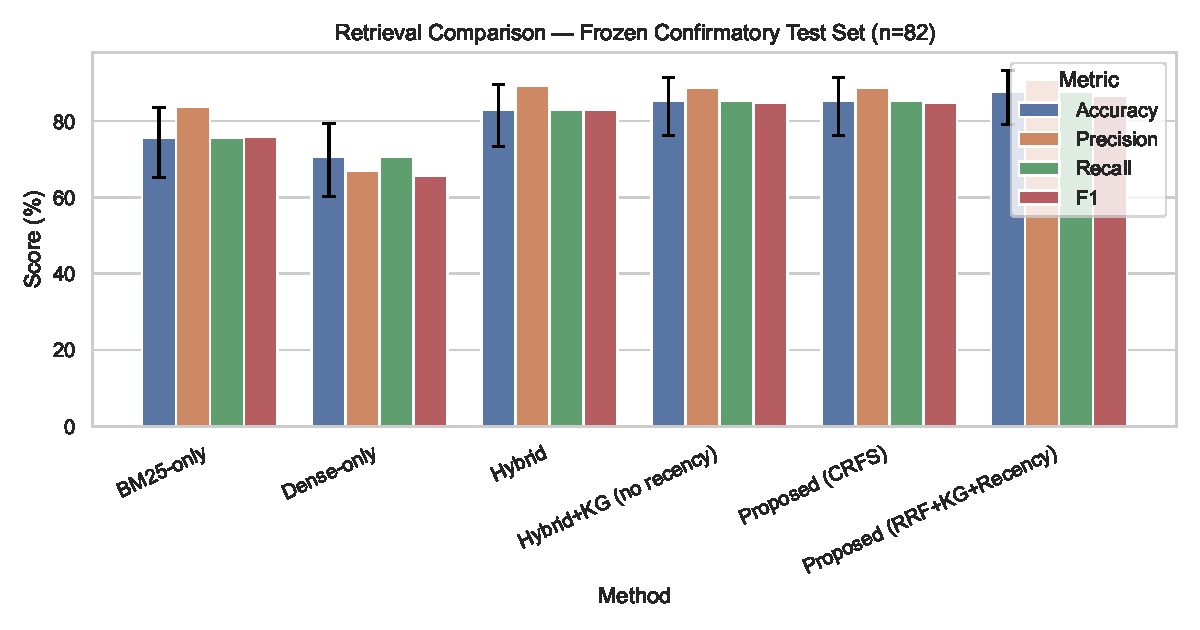
\includegraphics[width=\columnwidth]{figs/baseline_comparison.pdf}
\caption{Accuracy, precision, recall, and F1 across all six methods, with Wilson 95\% confidence intervals on accuracy. CRFS, not the proposed pipeline, now leads on accuracy, precision, and F1.}
\label{fig:baseline}
\end{figure}

McNemar's exact test finds CRFS's advantage over the proposed pipeline nominally significant at $\alpha=0.05$ (11 discordant pairs favoring CRFS against 2, $p=0.0225$), as is Hybrid+KG's advantage (10 vs.\ 2, $p=0.0386$). Neither survives Bonferroni correction ($\alpha=0.0125$), so we treat the reversal as suggestive rather than conclusive. The two comparisons that do survive correction point the same direction in both analyses: the proposed pipeline remains significantly more accurate than the plain hybrid (12 vs.\ 1, $p=0.00342$) and than dense retrieval alone (24 vs.\ 5, $p=0.000546$). It is specifically the two comparisons against the stronger, KG-equipped baselines, the ones that failed to reach significance originally as well, whose \emph{direction} has reversed.

\subsection{Attribution: Pool Size vs.\ Fusion Rule}

Table~\ref{tab:attribution} decomposes the 7.31-point gap between CRFS and the proposed pipeline. Restricting CRFS to the same top-3 shortlist while holding its linear fusion rule fixed (N1) drops accuracy from 86.99\% (Hybrid+KG, full pool) to 80.49\%, a 6.51-point loss (bootstrap 95\% CI: [$-$11.38, $-$1.63]) that is itself significant (9 vs.\ 1, $p=0.0215$): pool size alone accounts for essentially the entire gap. Comparing N1 directly against the proposed pipeline, same pool but RRF instead of a linear sum, yields 1 discordant pair each way ($p=1.0$; bootstrap mean difference $-0.02$ points, 95\% CI: [$-2.44$, $2.44$]): at matched pool size the two fusion rules are statistically indistinguishable. Removing the recency tiebreak (N2) changes zero predictions out of 123 ($p=1.0$; bootstrap difference exactly 0.0). The CRFS-vs-proposed gap is therefore attributable to candidate-pool size, not to reciprocal rank fusion outperforming linear fusion, and recency's marginal contribution as a tiebreaker is negligible here.

\begin{table}[t]
\centering
\caption{Attribution ablation isolating candidate-pool size from fusion rule ($n=123$).}
\label{tab:attribution}
\footnotesize
\setlength{\tabcolsep}{3pt}
\begin{tabular}{lcccc}
\toprule
\textbf{Condition} & \textbf{Acc.\ (\%)} & \textbf{Pool} & \textbf{Fusion} & \textbf{Recency} \\
\midrule
Hybrid+KG (no rec.) & 86.99 & full (104) & linear & no \\
N1 (linear @ shortlist) & 80.49 & top-3 & linear & no \\
N2 (prop., no tiebreak) & 80.49 & top-3 & RRF & no \\
Proposed (RRF+KG+Rec) & 80.49 & top-3 & RRF & yes (tiebreak) \\
\bottomrule
\end{tabular}
\end{table}

\subsection{Canonical vs.\ Paraphrased Queries}

Table~\ref{tab:subset} and Fig.~\ref{fig:subset} report accuracy separately on the 41 canonical and 82 paraphrased queries. Our original report used this split to argue that RRF's advantage over linear fusion concentrates in lay-phrased queries, where dense retrieval matters most; that pattern does not hold under the corrected data. CRFS reaches 100\% accuracy on canonical and 81.71\% on paraphrased, matching or exceeding the proposed pipeline (95.12\% and 73.17\%) on both. CRFS and Hybrid+KG tie exactly on the paraphrased subset (67 of 82 correct for both), consistent with the attribution result: the advantage tracks candidate-pool size and KG reranking over the full corpus, not whether fusion is linear or rank-based, and not query phrasing specifically. N1 and N2 reproduce the proposed pipeline's subset accuracy exactly (95.12\% canonical, 73.17\% paraphrased).

\begin{table}[t]
\centering
\caption{Accuracy (\%) on canonical ($n=41$) vs.\ paraphrased ($n=82$) queries.}
\label{tab:subset}
\footnotesize
\setlength{\tabcolsep}{4pt}
\begin{tabular}{lcc}
\toprule
\textbf{Method} & \textbf{Canonical} & \textbf{Paraphrased} \\
\midrule
BM25-only & 87.80 & 54.88 \\
Dense-only & 73.17 & 60.98 \\
Hybrid & 87.80 & 63.41 \\
Hybrid+KG (no rec.) & 97.56 & 81.71 \\
\textbf{CRFS} & \textbf{100.00} & \textbf{81.71} \\
Proposed (RRF+KG+Rec) & 95.12 & 73.17 \\
\bottomrule
\end{tabular}
\end{table}

\begin{figure}[t]
\centering
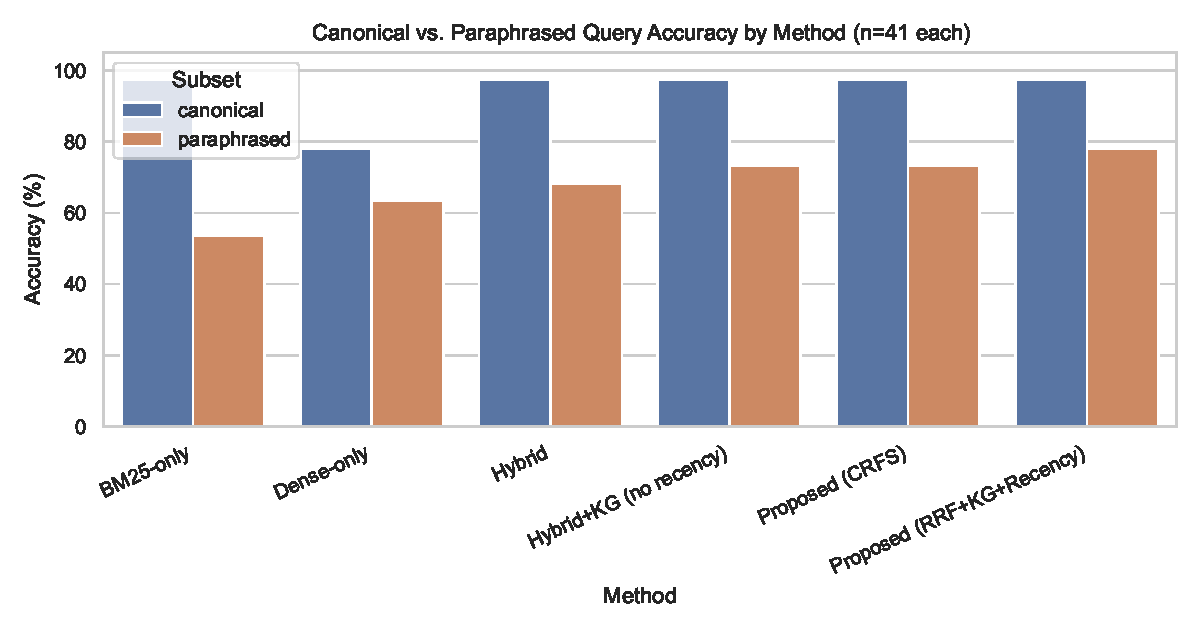
\includegraphics[width=\columnwidth]{figs/subset_breakdown.pdf}
\caption{Accuracy on canonical vs.\ paraphrased queries by method. CRFS leads on both subsets; the gap no longer narrows monotonically toward the proposed pipeline as it did in our original report.}
\label{fig:subset}
\end{figure}

\subsection{Latency}

Table~\ref{tab:main} (rightmost column) and Fig.~\ref{fig:accvlat} report mean latency on an NVIDIA RTX~3050 GPU under the corrected $n=123$ protocol. The proposed pipeline remains fastest among the four competitive (KG-equipped or hybrid) methods, at 21.25~ms against 72.66~ms for CRFS (3.4$\times$) and 35.59~ms for Hybrid+KG (1.7$\times$). In our original report, we attributed CRFS's latency cost to a recency term whose weight tuning had driven to zero. That explanation no longer holds: the corrected weights give recency a nonzero coefficient (0.103). The gap instead has the explanation Section~\ref{sec:results}A points to directly: CRFS scores KG relevance and recency across the full 104-document corpus on every query, while the proposed pipeline scores the same signals across only a 3-document shortlist, a real, structural difference in workload rather than the removal of wasted computation.

\begin{figure}[t]
\centering
\includegraphics[width=\columnwidth]{figs/accuracy_vs_latency.pdf}
\caption{Accuracy vs.\ mean GPU-synchronized latency, with error bars showing $\pm1$ standard deviation on latency. CRFS is the most accurate configuration and the most expensive; the proposed pipeline trades 7.3 accuracy points for a 3.4$\times$ latency reduction.}
\label{fig:accvlat}
\end{figure}

Framed against the two architectures under direct comparison, the result is an honest trade-off rather than a win for either side: CRFS is more accurate and slower, the proposed pipeline is less accurate and substantially faster, and neither dominates the other on both axes simultaneously.

\section{Discussion}

The central finding here is not that reciprocal rank fusion is a weaker combination rule than a linear sum, nor the reverse; the attribution ablation shows the two are statistically indistinguishable once candidate-pool size is held fixed (Section~\ref{sec:results}A). The finding is that our original weight-collapse result, and the architectural narrative built on it, was an artifact of a leaky evaluation protocol rather than a general property of linear fusion. Under a corrected, disjoint train/test split, the same weight search that previously collapsed to two zero-weight signals instead distributes weight across all four, and the accuracy ordering between the two architectures reverses. We lack a controlled experiment isolating the precise mechanism connecting the leakage to that degenerate solution; a plausible hypothesis is that a small, non-disjoint validation pool produced near-ties among candidate weight configurations that a fully held-out split no longer produces, but we flag this as a hypothesis, not a demonstrated mechanism.

The paraphrase-subgroup result (Section~\ref{sec:results}B) shows the same pattern: our hypothesis that dense retrieval's value would surface specifically on lay-phrased queries once a weight search could no longer suppress it does not survive the corrected data. CRFS matches or exceeds every configuration on both subsets, including the proposed pipeline. This does not mean dense retrieval is unhelpful; Dense-only alone reaches only 65.04\% accuracy, well below every KG-equipped configuration, and the proposed pipeline's advantage over the plain BM25+Dense hybrid remains significant after Bonferroni correction. What the corrected data does not support is the more specific claim that RRF's use of dense retrieval outperforms linear fusion's use of the same signal, at this sample size.

The pool-size finding is, we think, the genuinely useful positive result of this repair cycle. Restricting a linear, KG-reranked pipeline from the full corpus to a 3-document shortlist costs 6.5 accuracy points, significant at $n=123$; changing only the fusion rule while holding the shortlist fixed costs nothing measurable. How many candidates survive to reranking appears to matter more than which rule produced that shortlist. Whether this generalizes beyond medical retrieval, or beyond this corpus, is a question our sample size cannot answer; we present it as a testable hypothesis, not an established property of reranking pipelines in general.

\section{Limitations}

The corrected evaluation is intentionally controlled rather than a population-level clinical validation. The frozen test set contains 123 queries across 41 conditions (41 canonical, 82 paraphrased); the 104-passage guideline corpus has no verifiable source date for 31 passages (29.8\%), limiting recency's contribution regardless of architecture. Eight conditions were excluded from the development-validation tuning split for insufficient rows (Section~\ref{ssec:protocol}); this does not affect the confirmatory test set. Two of our four confirmatory comparisons (CRFS vs.\ proposed, Hybrid+KG vs.\ proposed) are nominally significant at $\alpha=0.05$ but not after Bonferroni correction; at this sample size we cannot rule out a false positive here, and we report both figures rather than only the one that clears correction. We disclose plainly that this paper's central comparison does not replicate our originally reported result: under the leaky v2 protocol the proposed pipeline was reported as more accurate, with the linear baseline degenerating to a two-signal system; under the corrected v3 protocol, the linear baseline uses all four signals and is more accurate, though not conclusively so after correction. Finally, the queries are synthetically constructed rather than patient-authored, and the sample, while larger than our original 82-query test set, remains modest for detecting small differences with high power. Larger guideline collections, naturally occurring queries, and a larger sample would each strengthen these conclusions.

\section{Conclusion}

We reported a finding from an earlier phase of this project, that a linearly fused retrieval baseline collapses to zero weight on two of four intended signals, that does not replicate under a corrected, leak-free protocol. Once the frozen test set is constructed as the genuine complement of the tuning pool, the same weight search distributes meaningful weight across all four signals, and the linear-fusion baseline (87.80\%) outperforms the reciprocal-rank-fusion pipeline we had proposed to replace it (80.49\%), a reversal that is nominally but not conclusively significant. A dedicated ablation traces this gap to candidate-pool size rather than fusion-rule choice: restricting the linear baseline to the proposed pipeline's top-3 shortlist reproduces its accuracy almost exactly, while the fusion rule itself makes no detectable difference at matched pool size. The proposed pipeline's latency advantage persists and remains genuine, a consequence of reranking fewer candidates rather than avoiding wasted computation on an unused signal. We present this trade-off, and the non-replication that led us to it, as the honest results of this repair cycle, and believe it is a stronger contribution than the narrative we originally set out to support. Future work includes larger guideline collections, patient-authored queries, a larger confirmatory sample to adjudicate the two comparisons left ambiguous after correction, and testing whether this pattern generalizes beyond medical retrieval.

\footnotesize
\begin{thebibliography}{00}

\bibitem{robertson2009bm25}
S.~Robertson and H.~Zaragoza, ``The Probabilistic Relevance Framework: BM25 and Beyond,'' \emph{Foundations and Trends in Information Retrieval}, vol.~3, no.~4, pp.~333--389, 2009.

\bibitem{karpukhin2020dpr}
V.~Karpukhin, B.~O\u{g}uz, S.~Min, P.~Lewis, L.~Wu, S.~Edunov, D.~Chen, and W.~Yih, ``Dense Passage Retrieval for Open-Domain Question Answering,'' in \emph{Proc.\ EMNLP}, 2020.

\bibitem{lewis2020rag}
P.~Lewis, E.~Perez, A.~Piktus, F.~Petroni, V.~Karpukhin, N.~Goyal, H.~K\"uttler, M.~Lewis, W.~Yih, T.~Rockt\"aschel, S.~Riedel, and D.~Kiela, ``Retrieval-Augmented Generation for Knowledge-Intensive NLP Tasks,'' in \emph{Proc.\ NeurIPS}, 2020.

\bibitem{cormack2009rrf}
G.~V.~Cormack, C.~L.~A.~Clarke, and S.~Buettcher, ``Reciprocal Rank Fusion Outperforms Condorcet and Individual Rank Learning Methods,'' in \emph{Proc.\ SIGIR}, 2009.

\bibitem{jin2023medcpt}
Q.~Jin, W.~Kim, Q.~Chen, D.~C.~Comeau, L.~Yeganova, W.~J.~Wilbur, and Z.~Lu, ``MedCPT: Contrastive Pre-trained Transformers with Large-scale PubMed Search Logs for Zero-shot Biomedical Information Retrieval,'' \emph{Bioinformatics}, vol.~39, no.~11, 2023.

\bibitem{devlin2019bert}
J.~Devlin, M.-W.~Chang, K.~Lee, and K.~Toutanova, ``BERT: Pre-training of Deep Bidirectional Transformers for Language Understanding,'' in \emph{Proc.\ NAACL-HLT}, 2019.

\bibitem{reimers2019sbert}
N.~Reimers and I.~Gurevych, ``Sentence-BERT: Sentence Embeddings using Siamese BERT-Networks,'' in \emph{Proc.\ EMNLP-IJCNLP}, 2019.

\bibitem{mcnemar1947}
Q.~McNemar, ``Note on the Sampling Error of the Difference Between Correlated Proportions or Percentages,'' \emph{Psychometrika}, vol.~12, no.~2, pp.~153--157, 1947.

\bibitem{wilson1927}
E.~B.~Wilson, ``Probable Inference, the Law of Succession, and Statistical Inference,'' \emph{Journal of the American Statistical Association}, vol.~22, no.~158, pp.~209--212, 1927.

\bibitem{efron1993bootstrap}
B.~Efron and R.~J.~Tibshirani, \emph{An Introduction to the Bootstrap}. Chapman \& Hall/CRC, 1993.

\bibitem{bora2024}
A.~Bora and H.~Cuay\'ahuitl, ``Systematic Analysis of Retrieval-Augmented Generation-Based LLMs for Medical Chatbot Applications,'' \emph{Machines}, vol.~6, no.~4, 2024.

\bibitem{shin2025}
M.~Shin, J.~Song, M.-G.~Kim, H.~W.~Yu, E.~K.~Choe, and Y.~J.~Chai, ``Thyro-GenAI: A Chatbot Using Retrieval-Augmented Generative Models for Personalized Thyroid Disease Management,'' \emph{Journal of Clinical Medicine}, vol.~14, no.~7, 2025.

\bibitem{lachenmayer2026}
H.~Lachenmayer, ``ClinicBot: A Guideline-Grounded Clinical Chatbot with Prioritized Evidence RAG and Verifiable Citations,'' \emph{arXiv preprint}, 2026.

\bibitem{nikam2024}
D.~S.~Nikam, D.~N.~Murthy, S.~Pragada, and H.~R.~Mamatha, ``BGKnow-Medical Chatbot: A Hybrid Approach Based on Knowledge Graph and GPT-2,'' \emph{Springer}, 2024.

\bibitem{putra2025}
P.~K.~Putra, E.~Nurfadhilah, S.~Pebiana, and E.~Prakasa, ``Towards a Safe and Trustworthy LLM-RAG Chatbot for Hemodialysis Patient Education: Design, Implementation, and Preliminary Evaluation,'' \emph{IEEE/ResearchGate}, 2025.

\bibitem{ruhland2026}
J.~B.~Ruhland, D.~Bahcivan, J.-P.~Sowa, A.~Canbay, and D.~Heider, ``MedChat: A Fully Offline Multimodal AI System for Privacy-Preserving Clinical Anamnesis,'' \emph{Frontiers in Artificial Intelligence}, 2026.

\end{thebibliography}

\end{document}
